%%%%%%%%%%%%%%%%%%%%%%%%%%%%%%%%%%%%%%%%%%%%%%%%%%%%%%%%%%%
% --------------------------------------------------------
% Tau
% LaTeX Template
% Version 2.4.1 (22/05/2024)
%
% Author: 
% Guillermo Jimenez (memo.notess1@gmail.com)
% 
% License:
% Creative Commons CC BY 4.0
% --------------------------------------------------------
%%%%%%%%%%%%%%%%%%%%%%%%%%%%%%%%%%%%%%%%%%%%%%%%%%%%%%%%%%%
\documentclass[9pt,a4paper,twoside]{tau-class/tau}

%----------------------------------------------------------
% TITLE
%----------------------------------------------------------

\journalname{计算物理\uppercase\expandafter{\romannumeral3}}
\title{快速傅里叶变换}

%----------------------------------------------------------
% AUTHORS, AFFILIATIONS AND PROFESSOR
%----------------------------------------------------------

\author[a,1]{Author}
%\author[b,2]{Author Two}
%\author[b,c,3]{Author Three}

%----------------------------------------------------------

\affil[a]{武汉大学,物理科学与技术学院}
%\affil[b]{Affiliation of author two}
%\affil[c]{Affiliation of author three}

%\professor{Professor/Authority or other information}

%----------------------------------------------------------
% FOOTER INFORMATION
%----------------------------------------------------------

\institution{Wuhan University}
\footinfo{Homework\uppercase\expandafter{\romannumeral2}}
\theday{November, 2024}
\leadauthor{Author}
\course{计算物理\uppercase\expandafter{\romannumeral3}}

%----------------------------------------------------------
% ABSTRACT AND KEYWORDS
%----------------------------------------------------------

\begin{abstract}    

\end{abstract}

%----------------------------------------------------------

\keywords{快速傅里叶变换,贝塞尔函数,Python}

%----------------------------------------------------------
\begin{document}
		
    \maketitle 
    \thispagestyle{firststyle}
	%\tauabstract 
    \taukeywords
    \tableofcontents
    \linenumbers 
    
%----------------------------------------------------------

\section{Introduction}
数学物理中最常出现的主题是傅里叶分析。例如,它出现在经典力学和非简正模的分析中,出现在电磁理论和波的频率分析中,出现在噪声考虑和热物理中,出现在量子理论和动量与坐标表示之间的转换中,出现在相对论量子场论中,出现在非正则态的产生和湮灭运算中.\cite{Ha}在介绍快速傅里叶变换的算法之前,我们首先简单回顾一下傅里叶变换的定义。
\subsection{傅里叶级数}
在关于贝塞尔函数的迭代计算作业中,我们提到了魏尔斯特拉斯定理,它告诉我们任意关于x的连续函数都可以展开成x的代数多项式。这个结论可以推广到n个自变量的情形:
\begin{tauenv}[frametitle=Generalized Stone-Weierstrass Theorem]
如果函数$f(x_1,x_2,\cdots,x_n)$是区间$[a_i,b_i]^n$上的连续函数,那么$f(x_1,x_2,\cdots,x_n)$可以展开成多项式$x_1^{k_1}x_2^{k_2}\cdots x_n^{k_n},k_i\text{是非负整数}$.
\end{tauenv}
由$x=r\cos\theta,y=r\sin\theta$,我们得到了极坐标下展开一个二元函数的方法:
\begin{align}
    f(r,\theta)=\sum_{m,k=0}^{\infty}a_{mk}x^ky^m=\sum_{m,k=0}^{\infty}a_{m,k}r^{m+k}\cos^k\theta\sin^m\theta
\end{align}
如果我们令$r=1$(或者其他常数)就得到了一个只关于$\theta$的函数:
\begin{align}
    f(\theta)=\sum_{n=-\infty}^{\infty}b_ne^{in\theta}
    =b_0+\sum_{n=1}^{\infty}(A_n\cos\theta+B_n\sin\theta)
\end{align}
这是一个周期为$2\pi$的周期性函数,它可以表示$[-\pi,\pi]$上的连续函数(或者分段连续函数,准确地讲是满足狄利克雷条件的函数)。
利用正交性和归一性,不难求出\cite{Ha}
\begin{align}
b_n=\frac{1}{\sqrt{2\pi}}\int_{-\pi}^{\pi}e^{-in\theta}f(\theta) \dd{\theta}
\end{align}
但是,我们感兴趣的函数并不总是定义在$(-\pi,\pi)$上。更一般的,对于定义在$(a,b)$上,周期为L=(b-a)的函数F(x),通过换元
\begin{align*}
    \theta =\frac{2\pi}{L}(x-a-\frac{L}{2})
\end{align*}
可以得到
\begin{align}
    &F(x)=\frac{1}{\sqrt{L}}\sum_{-\infty}^{\infty}F_n e^{2\pi inx/L}\\
    &F_n=\frac{1}{\sqrt{L}}\int_{a}^{b}e^{-2\pi inx/L}F(x)\dd{x}
\end{align}
\subsection{傅里叶变换}
傅里叶级数可以展开任意周期性函数F(x),但是物理学中遇到的大多数函数并不是周期性的。
\begin{figure}
    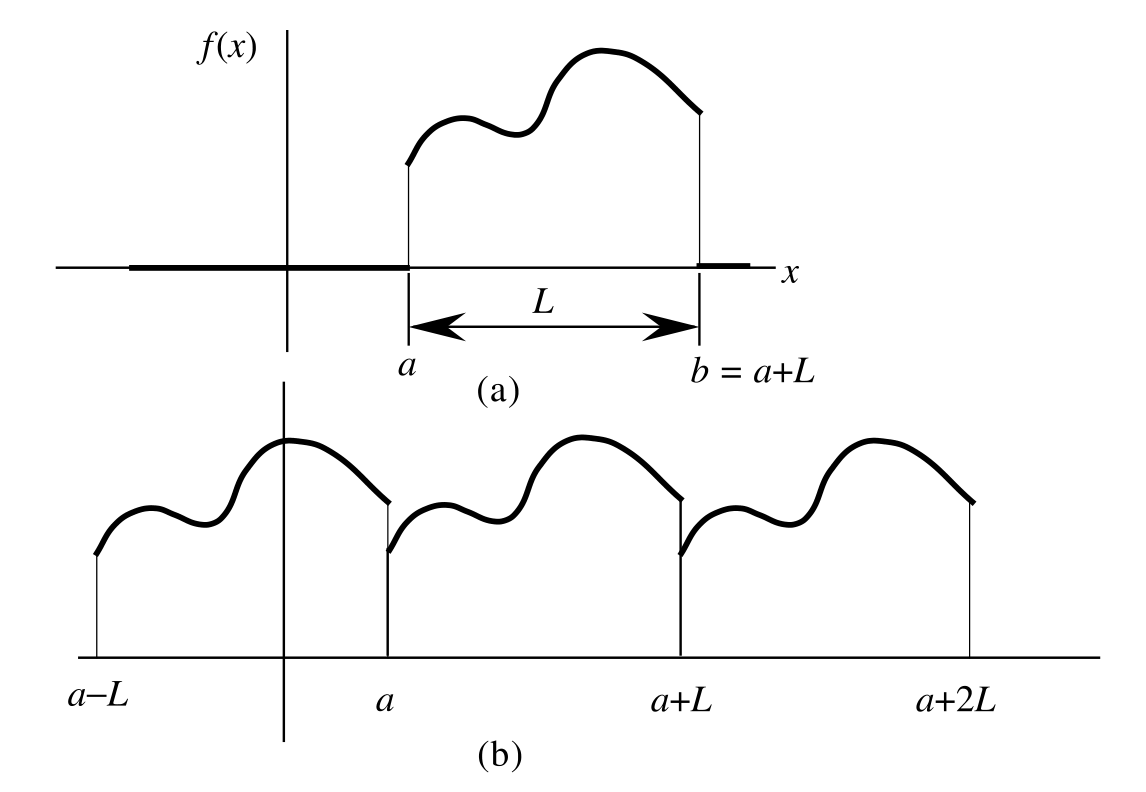
\includegraphics[width=\linewidth]{figures/FFT0}
    \caption{(a) The function we want to represent. (b) The Fourier series representation of
    the function}
\end{figure}
一种简单的想法是使周期$L\rightarrow \infty$,此时$\Delta\omega=\frac{2\pi}{L}\rightarrow 0$。\cite{MP}我们直接给出傅里叶积分的定义,为了避免和频率f混淆,我们改用h(t)表示函数。
\begin{align}
    H(\omega)=\int_{-\infty}^{\infty} h(t)e^{i\omega t}\dd{t}\\
    h(t)=\frac{1}{2\pi}\int_{-\infty}^{\infty}H(\omega)e^{-i\omega t}\dd{\omega}
\end{align}
\section{快速傅里叶变换}
\subsection{Sampling Theorem and Aliasing}
在通常情况下,h(t)是通过均匀采样得到的,令$\Delta$表示两次相邻采样的时间间隔,称为采样率(sample rate)。
对任何采样率$\Delta$,有一个相对应的临界频率,称为Nyquist临界频率(Nyquist critical frequency)\cite{Numerical}
\begin{equation}
    f_c=\frac{1}{2\Delta}
\end{equation}
关于二者有一个重要的定理:
\begin{tauenv}[frametitle=sampling theorem]
    If a continuous function h(t), sampled at an
interval $\Delta$, happens to be $bandwidth$ limited to frequencies smaller in magnitude than
$f_c$, i.e., if $H(f) = 0$ for all $|f| \geq  f_c$, then the function h(t) is completely determined
by its samples $h_n$.
\end{tauenv}
\subsection{离散傅里叶变换(Discrete Fourier Transform)}
对于周期为无穷的函数h(t),我们只需要对有限的的部分进行采样(h(t)等于零的部分积分仍然是0),我们将h(t)开始的初始时刻记为$t=0$,
\begin{align}
    h_k=h(k\Delta),\qquad k=0,1,\cdots,N-1
\end{align}
利用这N个输入的$h_k$,我们可以得到
\begin{align}
    H(f_n)=\int_{-\infty}^{\infty} h(t)e^{2\pi i f_n t}\dd{t}=\int_{0}^{(N-1)\Delta} e^{2\pi f_n k\Delta}\dd{t}    
\end{align}
根据前面的叙述,为了将h(t)用$h(t)=\frac{1}{2\pi}\int_{-\infty}^{\infty}H(\omega)e^{-i\omega t}\dd{\omega}$表示,h(t)的周期看作无穷,$\Delta\omega=\frac{2\pi}{L}\rightarrow 0$,我们应当取无数个$f_n$的值。在推导傅里叶积分的过程中,这当然是没有问题的,$\Delta\omega=\frac{2\pi}{L}\rightarrow 0$意味着求和被积分所取代,但当我们实际进行数值计算时却不能取无穷个$f_n$。出于对称性的考虑,我们同样也取N个$f_n$的值,这样可以重复利用一部分代码
\begin{align}
    f_n=\frac{n}{N\Delta},\qquad n=-\frac{N}{2},\cdots,\frac{N}{2}
\end{align}
这样$f_n$刚好均匀分布在$-f_c,f_c$。$f_n$取更大的值没有意义,因为如采样定理所描述,在当前的$\Delta$下,提取不到更高频率的信号的信息(从实际操作过程看,我们的$\Delta$是根据信号中存在的频率的上限选取的,$f_c$是采样的信号中存在的最大的频率,信号中本来不具备比$f_c$频率更高的信号)。\\
引入记号$H_n=H(f_n)\Delta$。
\begin{align}
H_n=\sum_{k=0}^{N-1}h_k e^{2\pi ikn/N}=\sum_{k=0}^{N-1}h_k W_N^{nk}\label{N2}
\end{align}
其中$W_N=e^{2\pi i/N}$不难验证$H_{-n}=H_{N-n}$,所以
\begin{align}
    h_k=\frac{1}{N}\sum_{n=0}^{N-1}H_ne^{-2\pi ikn/N}
\end{align}
\subsection{快速傅里叶变换(Fast Fourier Transform)}
由公式\ref{N2}可知,进行离散傅里叶变换相当于一个$N\times N$矩阵和一个N维向量相乘,所需要的时间为$O(N^2)$,利用单位复数根的性质可以将时间缩短为$O(N\log{N})$\cite{suan}。
\begin{tauenv}[frametitle=单位复数根]
    单位复数根是满足$W^N=1$的复数$W$,这样的复数刚好有N个,$e^{2\pi in/N},n=0,1,\cdots,N-1$。它们均匀地分布在以原点为中心的单位圆上。$W_N=e^{2\pi i/N}$称呼为N次主单位根。其它根都是$W_N$的幂。
\end{tauenv}
\begin{figure}[h]
    \centering
    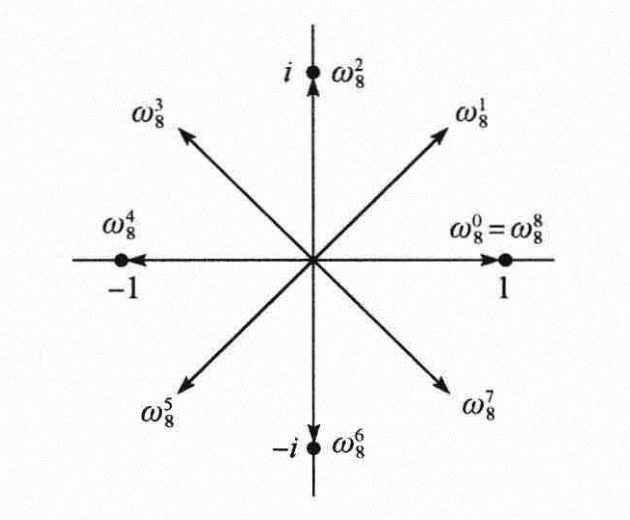
\includegraphics[width=\linewidth]{figures/FFT1}
    \caption{8次单位复数根}
\end{figure}
N个N次单位复数根以乘法为群乘法构成一个群,与加法群同构,我们给出单位复数根的几个基本性质:
\begin{enumerate}
    \item $W_N^jW_N^k=W_N^{j+k}=W_N^{(j+k)\mod N}$
    \item 消去引理:$W_{mN}^{mk}=W_N^k$
    \item 折半引理:N个N次单位复数根的平方的集合就是N/2个N/2次单位复数根的集合:$W_N^{k+N/2}=-W_N^k,(W_N^k)^2=W_{N/2}^k$
\end{enumerate}

现在回到计算$H_n$的问题上。我们采取分治策略,利用$H_n$的偶数项(even)和奇数项(odd)分别定义$H^e$和$H^o$.
\begin{equation}
    \begin{aligned}
        H_n(h,W_N^n)=&h_0+W_N^{n}h_1+W_N^{2n}h_2+\cdots+W_N^{(N-1)n}h_{N-1}\\
            =&(h_0+W_N^{2n}h_2+\cdots+W_N^{(N-2)n}h_{N-2})+\\
            &W_N^n(h_1+W_N^{2n}h_3+\cdots+W_N^{(N-2)n}h_{N-1})\\
            =&H_n(h^e,W_{N/2}^n)+W_N^nH_n(h^o,W_{N/2}^n)\\
            =&H_n^e+W_N^nH_n^o
    \end{aligned}
\end{equation}
这样就把求$H_n,n=0,1,2,\cdots,N-1$的问题转化为求$H_n^e$和$H_n^o,n=0,1,2,\cdots,N/2-1$的问题。(折半引理)。这两个子问题的形式与原始问题相同。重复以上步骤,我们可以得到:(一个元素的DFT就是它自身)
\begin{align}
    H^{eoooee\cdots}_n=h_k
\end{align}
那么,n和k之间有什么关系呢?我们来回顾刚刚的过程,$h_k$被归入$H^e$系数的原因是k是偶数,将k写成二进制,k的末位是0;而末位是1的k对应的$h_k$则被归入$h^o$。然后对分出的两组,重复以上过程,看第二末位是0还是1。这个过程和判断二进制数的大小是相似的,当我们判断二进制数大小时,首先看最高位是0还是1,然后将所有数分为较小的半组和较大的半组,然后对第二高位重复这个过程。因此我们只需要将k转为二进制,然后左右翻转,对$bit\_rev(k)$按大小进行排序。
\begin{figure}[h]
    \centering
    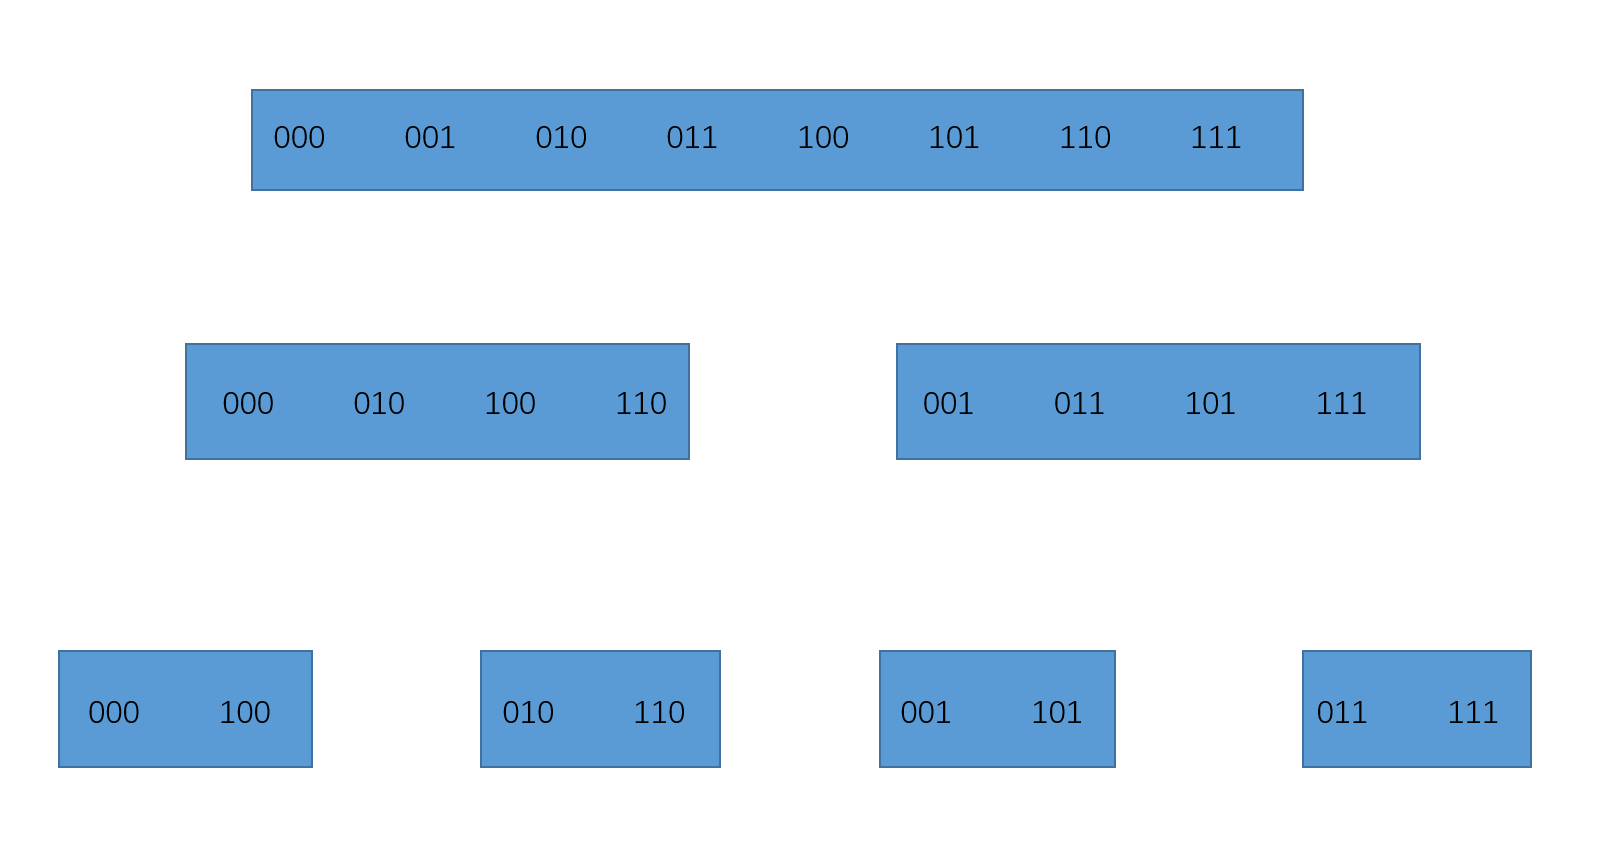
\includegraphics[width=\linewidth]{figures/FFT2}
    \caption{对$2^M$个数按奇偶划分直至每组只有一个,相当于将下标按二进制反转,并从小到大排列}
\end{figure}
在对$h_k$在二进制倒序之后,就可以按照迭代结构而不是递归结构计算。
\begin{figure*}[h]
    \centering
    \begin{subfigure}{0.3\linewidth}
        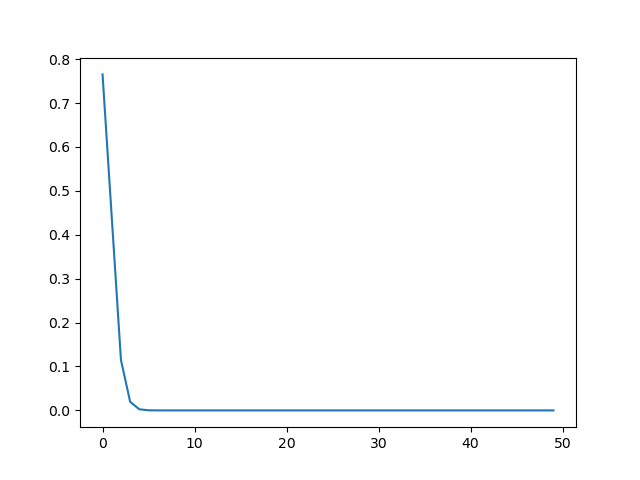
\includegraphics[width=\linewidth]{figures/result1.png}
    \end{subfigure}
    \begin{subfigure}{0.3\linewidth}
        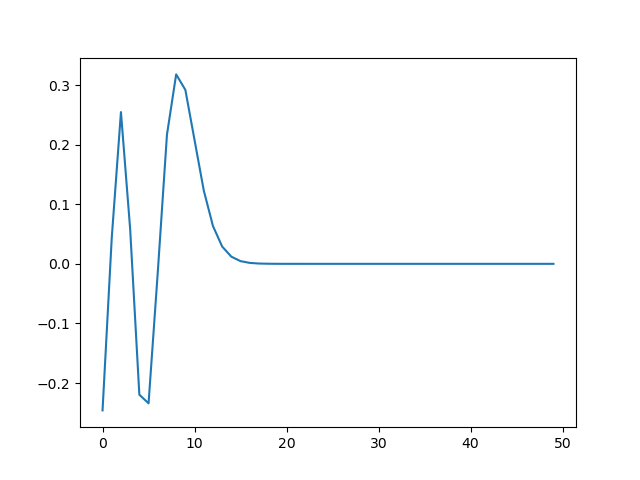
\includegraphics[width=\linewidth]{figures/result10.png}
    \end{subfigure}
    \begin{subfigure}{0.3\linewidth}
        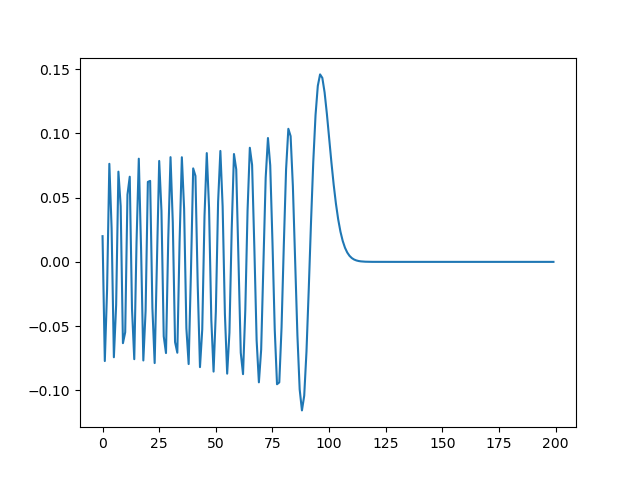
\includegraphics[width=\linewidth]{figures/result100.png}
    \end{subfigure}
    \caption{z = 1, 10 and 100时的$J_n(z)$}
\end{figure*}
\begin{figure}[h]
    \centering
    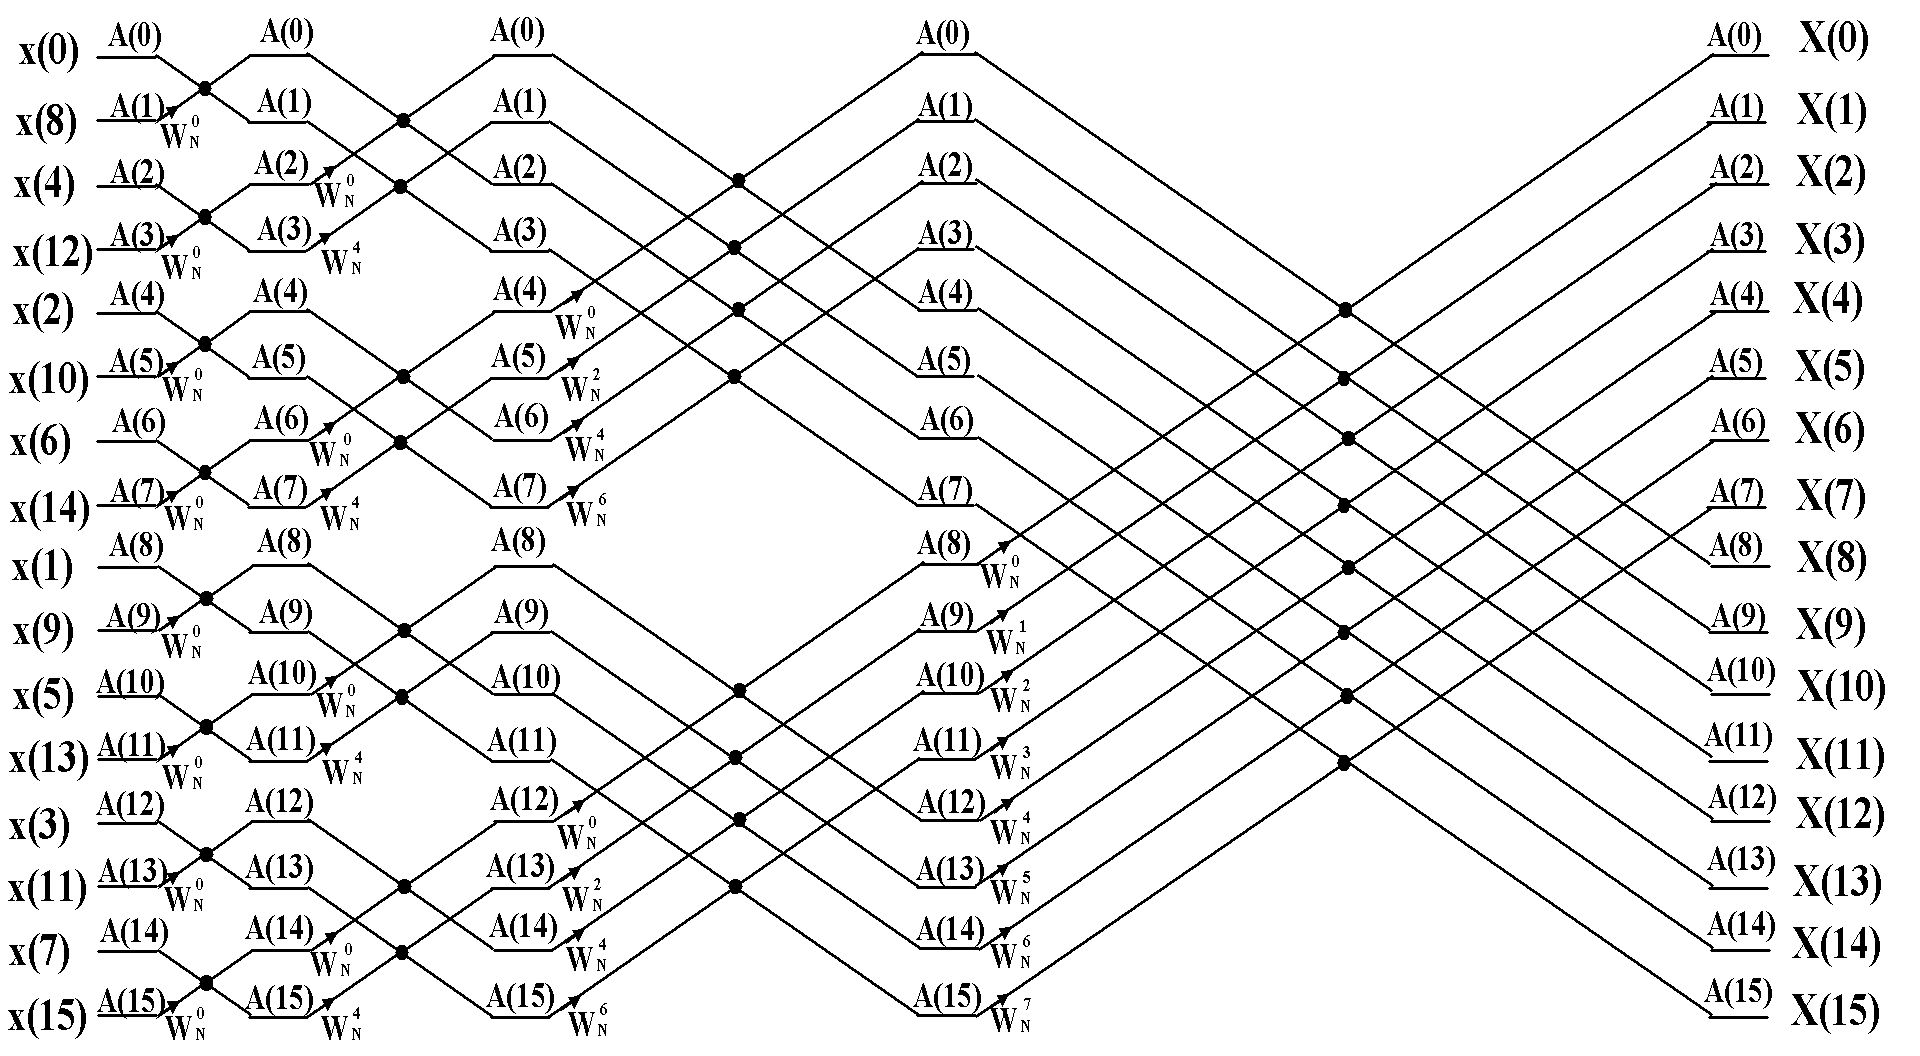
\includegraphics[width=\linewidth]{figures/4.jpg}
    \caption{在二进制倒序之后,就可以按照迭代结构而不是递归结构计算。}
\end{figure}
N=$2^M$时要进行蝶形运算,我们要解决的问题有:
\begin{enumerate}
    \item 两个输入数据之间的间隔B
    \item 旋转因子W的确定,包括:
    \begin{enumerate}
        \item 第L级旋转指数
        \item 第L级W的种类确定
        \item 第L级中同一W之间的间隔
    \end{enumerate}
\end{enumerate}
观察蝶形图可知第L级:
\begin{enumerate}
    \item 两个输入数据间距为$B=2^{l-1}$
    \item 有$2^{L-1}$个旋转因子
    \item 旋转因子W增量为$2^{M-L}$
    \item 同一W间隔为$istep=2B=2^L$
    \item 同种蝶形运算次数为$2^{M-L}$
\end{enumerate}
\section{使用FFT算法计算Bessel函数}
利用FFT程序可以按照如下的积分计算Bessel函数:
\begin{tauenv}[frametitle=Bessel function]
    \begin{align}
        J_n(z)=\frac{i^{-n}}{2\pi}\int^{2\pi}_0 e^{izcos\theta }e^{in\theta }d\theta 
    \end{align}
\end{tauenv}
Bessel函数的积分可以写成如下的FFT形式:
\begin{align}
    J_n(z)=&\frac{i^{-n}}{N}\sum\limits^{N-1}_{k=0} e^{izcos(2\pi k/N) }e^{2\pi ink/N}\notag\\
    &=\frac{i^{-n}}{N}H_n[e^{izcos(2\pi k/N) },W^n_N]
\end{align}
\newpage
\section{Codes}
	\nolinenumbers
	\lstinputlisting[caption=code, language=Matlab]{main.py}
	\linenumbers





%\clearpage%新一页而不是新一列

	
%    If line numbering is enabled, we recommend placing the command \verb|\nolinenumbers| at the beginning %and \verb|\linenumbers| at the end of the code. 
%	
%    This will temporarily remove line numbering and the code will look better as shown in this example.

%----------------------------------------------------------
\nocite{*}
\addcontentsline{toc}{section}{References}

\printbibliography

%----------------------------------------------------------
%\section{Document style options}
%
%    \subsection{Tau start}
%	
%        We included the \verb|\taustart{}| command, which provides a personalized lettrine for the %beginning of a paragraph.
%
%    \subsection{Line numbering}
%	
%        By implementing the \textit{lineno} package, the line numbering of the document can be placed with %the command \verb|\linenumbers|.
%		
%        I recommend placing the command after the abstract and table of contents for a better appearance.
%		
%    \subsection{Table of contents}
%	
%        The \textit{tau class} provides a customised design for the table of contents. Each level of the %ToC provides a preview of the content and its location in the document. 
%		
%section{Figures and tables}
%
%   \subsection{Figures}
%		
%	Fig. \ref{fig:figure} shows an example figure.
%		
%	\begin{figure}[H]
%		\centering
%		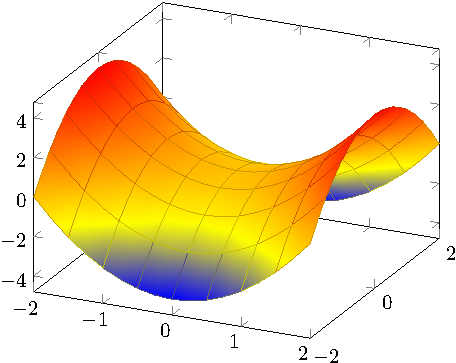
\includegraphics[width=0.75\columnwidth]{figures/Example.pdf}
%		\caption{Example figure obtained from PGFPlots \cite{PFGPlots}.}
%		\label{fig:figure}
%	\end{figure}
%		
%       Fig. \ref{fig:examplefloat} shows an example of two figures that covers the width of the page. It can be placed at the top or bottom of the page. The space between the figures can also be changed using the \verb|\hspace{Xpt}| command.
%		
   
	
%    \subsection{Tables}
%	
%        Table \ref{tab:table} shows an example table. The \verb|\tabletext{}| is used to add notes to %tables easily. 
%		
%	\begin{table}[H]
%		\centering
%		\caption{Small example table.}
%		\label{tab:table}
%		\begin{tabular}{cc}
%			\toprule
%			\textbf{Column 1} & \textbf{Column 2} \\
%			\midrule
%			Data 1 & Data 2 \\
%			Data 3 & Data 4 \\
%			\bottomrule
%		\end{tabular}
%			
%            \tabletext{Note: I'm a table text for additional information.}
%			
%	\end{table}
%		
%\section{Tau packages}
%
%    \subsection{Tauenvs}
%	
%		
%	\begin{tauenv}[frametitle=Environment with custom title]
%            This is an example of the custom title environment. To add a title type \verb|[frametitle=Your %title]| next to the beginning of the environment (as shown in this example).
%	\end{tauenv}
%
%		
%\section{Equation}
%
%    Equation \ref{ec:equation}, shows the Schrödinger equation as an example. 
%	\begin{equation} \label{ec:equation}
%		\frac{\hbar^2}{2m}\nabla^2\Psi + V(\mathbf{r})\Psi = -i\hbar \frac{\partial\Psi}{\partial t}
%	\end{equation} 
\end{document}